\documentclass[a4paper]{article}

\usepackage[pdftex,
  hidelinks,
  pdfauthor={Dexter Chua},
  pdfsubject={Cambridge Maths Notes: Part IB - Variational Principles},
  pdftitle={Part IB - Variational Principles},
pdfkeywords={Cambridge Mathematics Maths Math IB Easter Variational Principles}]{hyperref}

\title{Part IB - Variational Principles}
\author{Lectured by P. K. Townsend}
\date{Easter 2015}

% Imports
\ifx \nextra \undefined
  \usepackage[pdftex,
    hidelinks,
    pdfauthor={Dexter Chua},
    pdfsubject={Cambridge Maths Notes: Part \npart\ - \ncourse},
    pdftitle={Part \npart\ - \ncourse},
  pdfkeywords={Cambridge Mathematics Maths Math \npart\ \nterm\ \nyear\ \ncourse}]{hyperref}
  \title{Part \npart\ - \ncourse}
\else
  \usepackage[pdftex,
    hidelinks,
    pdfauthor={Dexter Chua},
    pdfsubject={Cambridge Maths Notes: Part \npart\ - \ncourse\ (\nextra)},
    pdftitle={Part \npart\ - \ncourse\ (\nextra)},
  pdfkeywords={Cambridge Mathematics Maths Math \npart\ \nterm\ \nyear\ \ncourse\ \nextra}]{hyperref}

  \title{Part \npart\ - \ncourse \\ {\Large \nextra}}
\fi

\author{Lectured by \nlecturer \\\small Notes taken by Dexter Chua}
\date{\nterm\ \nyear}

\usepackage{alltt}
\usepackage{amsfonts}
\usepackage{amsmath}
\usepackage{amssymb}
\usepackage{amsthm}
\usepackage{booktabs}
\usepackage{caption}
\usepackage{enumitem}
\usepackage{fancyhdr}
\usepackage{graphicx}
\usepackage{mathtools}
\usepackage{microtype}
\usepackage{multirow}
\usepackage{pdflscape}
\usepackage{pgfplots}
\usepackage{siunitx}
\usepackage{tabularx}
\usepackage{tikz}
\usepackage{tkz-euclide}
\usepackage[normalem]{ulem}
\usepackage[all]{xy}

\pgfplotsset{compat=1.12}

\pagestyle{fancyplain}
\lhead{\emph{\nouppercase{\leftmark}}}
\ifx \nextra \undefined
  \rhead{
    \ifnum\thepage=1
    \else
      \npart\ \ncourse
    \fi}
\else
  \rhead{
    \ifnum\thepage=1
    \else
      \npart\ \ncourse\ (\nextra)
    \fi}
\fi
\usetikzlibrary{arrows}
\usetikzlibrary{decorations.markings}
\usetikzlibrary{decorations.pathmorphing}
\usetikzlibrary{positioning}
\usetikzlibrary{fadings}
\usetikzlibrary{intersections}
\usetikzlibrary{cd}

\newcommand*{\Cdot}{\raisebox{-0.25ex}{\scalebox{1.5}{$\cdot$}}}
\newcommand {\pd}[2][ ]{
  \ifx #1 { }
    \frac{\partial}{\partial #2}
  \else
    \frac{\partial^{#1}}{\partial #2^{#1}}
  \fi
}

% Theorems
\theoremstyle{definition}
\newtheorem*{aim}{Aim}
\newtheorem*{axiom}{Axiom}
\newtheorem*{claim}{Claim}
\newtheorem*{cor}{Corollary}
\newtheorem*{defi}{Definition}
\newtheorem*{eg}{Example}
\newtheorem*{fact}{Fact}
\newtheorem*{law}{Law}
\newtheorem*{lemma}{Lemma}
\newtheorem*{notation}{Notation}
\newtheorem*{prop}{Proposition}
\newtheorem*{thm}{Theorem}

\renewcommand{\labelitemi}{--}
\renewcommand{\labelitemii}{$\circ$}
\renewcommand{\labelenumi}{(\roman{*})}

\let\stdsection\section
\renewcommand\section{\newpage\stdsection}

% Strike through
\def\st{\bgroup \ULdepth=-.55ex \ULset}

% Maths symbols
\newcommand{\bra}{\langle}
\newcommand{\ket}{\rangle}

\newcommand{\N}{\mathbb{N}}
\newcommand{\Z}{\mathbb{Z}}
\newcommand{\Q}{\mathbb{Q}}
\renewcommand{\H}{\mathbb{H}}
\newcommand{\R}{\mathbb{R}}
\newcommand{\C}{\mathbb{C}}
\newcommand{\Prob}{\mathbb{P}}
\renewcommand{\P}{\mathbb{P}}
\newcommand{\E}{\mathbb{E}}
\newcommand{\F}{\mathbb{F}}
\newcommand{\cU}{\mathcal{U}}
\newcommand{\RP}{\mathbb{RP}}
\newcommand{\CP}{\mathbb{CP}}

\newcommand{\ph}{\,\cdot\,}

\DeclareMathOperator{\sech}{sech}
\DeclareMathOperator{\cosech}{cosech}
\DeclareMathOperator{\cosec}{cosec}

\DeclareMathOperator{\covol}{covol}
\DeclareMathOperator{\vol}{vol}

\let\Im\relax
\let\Re\relax
\DeclareMathOperator{\Im}{Im}
\DeclareMathOperator{\Re}{Re}
\DeclareMathOperator{\im}{im}
\DeclareMathOperator{\image}{image}
\DeclareMathOperator{\Ann}{Ann}

\DeclareMathOperator*{\res}{res}
\DeclareMathOperator{\Res}{Res}
\DeclareMathOperator{\Ind}{Ind}

\DeclareMathOperator{\tr}{tr}
\DeclareMathOperator{\diag}{diag}
\DeclareMathOperator{\rank}{rank}
\DeclareMathOperator{\card}{card}
\DeclareMathOperator{\spn}{span}
\DeclareMathOperator{\adj}{adj}

\DeclareMathOperator{\erf}{erf}
\DeclareMathOperator{\erfc}{erfc}

\DeclareMathOperator{\ord}{ord}
\DeclareMathOperator{\Sym}{Sym}

\DeclareMathOperator{\sgn}{sgn}
\DeclareMathOperator{\orb}{orb}
\DeclareMathOperator{\stab}{stab}
\DeclareMathOperator{\ccl}{ccl}

\DeclareMathOperator{\lcm}{lcm}
\DeclareMathOperator{\hcf}{hcf}

\DeclareMathOperator{\Int}{Int}
\DeclareMathOperator{\id}{id}

\DeclareMathOperator{\betaD}{beta}
\DeclareMathOperator{\gammaD}{gamma}
\DeclareMathOperator{\Poisson}{Poisson}
\DeclareMathOperator{\binomial}{binomial}
\DeclareMathOperator{\multinomial}{multinomial}
\DeclareMathOperator{\Bernoulli}{Bernoulli}
\DeclareMathOperator{\like}{like}

\DeclareMathOperator{\var}{var}
\DeclareMathOperator{\cov}{cov}
\DeclareMathOperator{\bias}{bias}
\DeclareMathOperator{\mse}{mse}
\DeclareMathOperator{\corr}{corr}

\DeclareMathOperator{\otp}{otp}
\DeclareMathOperator{\dom}{dom}

\DeclareMathOperator{\Root}{Root}
\DeclareMathOperator{\supp}{supp}
\DeclareMathOperator{\rel}{rel}
\DeclareMathOperator{\Hom}{Hom}
\DeclareMathOperator{\Aut}{Aut}
\DeclareMathOperator{\Gal}{Gal}
\DeclareMathOperator{\Mat}{Mat}
\DeclareMathOperator{\End}{End}
\DeclareMathOperator{\Char}{char}
\DeclareMathOperator{\ev}{ev}
\DeclareMathOperator{\St}{St}
\DeclareMathOperator{\Lk}{Lk}
\DeclareMathOperator{\disc}{disc}
\DeclareMathOperator{\Isom}{Isom}
\DeclareMathOperator{\length}{length}
\DeclareMathOperator{\energy}{energy}
\DeclareMathOperator{\area}{area}
\DeclareMathOperator{\Syl}{Syl}
\DeclareMathOperator{\cl}{cl}
\DeclareMathOperator{\fix}{fix}

\newcommand{\GL}{\mathrm{GL}}
\newcommand{\SL}{\mathrm{SL}}
\newcommand{\PGL}{\mathrm{PGL}}
\newcommand{\PSL}{\mathrm{PSL}}
\newcommand{\PSU}{\mathrm{PSU}}
\newcommand{\Or}{\mathrm{O}}
\newcommand{\SO}{\mathrm{SO}}
\newcommand{\U}{\mathrm{U}}
\newcommand{\SU}{\mathrm{SU}}

\renewcommand{\d}{\mathrm{d}}
\newcommand{\D}{\mathrm{D}}

\tikzset{->/.style = {decoration={markings,
                                  mark=at position 1 with {\arrow[scale=2]{latex'}}},
                      postaction={decorate}}}
\tikzset{<-/.style = {decoration={markings,
                                  mark=at position 0 with {\arrowreversed[scale=2]{latex'}}},
                      postaction={decorate}}}
\tikzset{<->/.style = {decoration={markings,
                                   mark=at position 0 with {\arrowreversed[scale=2]{latex'}},
                                   mark=at position 1 with {\arrow[scale=2]{latex'}}},
                       postaction={decorate}}}
\tikzset{->-/.style = {decoration={markings,
                                   mark=at position #1 with {\arrow[scale=2]{latex'}}},
                       postaction={decorate}}}
\tikzset{-<-/.style = {decoration={markings,
                                   mark=at position #1 with {\arrowreversed[scale=2]{latex'}}},
                       postaction={decorate}}}

\tikzset{circ/.style = {fill, circle, inner sep = 0, minimum size = 3}}
\tikzset{mstate/.style={circle, draw, blue, text=black, minimum width=0.7cm}}

\definecolor{mblue}{rgb}{0.2, 0.3, 0.8}
\definecolor{morange}{rgb}{1, 0.5, 0}
\definecolor{mgreen}{rgb}{0.1, 0.4, 0.2}
\definecolor{mred}{rgb}{0.5, 0, 0}

\def\drawcirculararc(#1,#2)(#3,#4)(#5,#6){%
    \pgfmathsetmacro\cA{(#1*#1+#2*#2-#3*#3-#4*#4)/2}%
    \pgfmathsetmacro\cB{(#1*#1+#2*#2-#5*#5-#6*#6)/2}%
    \pgfmathsetmacro\cy{(\cB*(#1-#3)-\cA*(#1-#5))/%
                        ((#2-#6)*(#1-#3)-(#2-#4)*(#1-#5))}%
    \pgfmathsetmacro\cx{(\cA-\cy*(#2-#4))/(#1-#3)}%
    \pgfmathsetmacro\cr{sqrt((#1-\cx)*(#1-\cx)+(#2-\cy)*(#2-\cy))}%
    \pgfmathsetmacro\cA{atan2(#2-\cy,#1-\cx)}%
    \pgfmathsetmacro\cB{atan2(#6-\cy,#5-\cx)}%
    \pgfmathparse{\cB<\cA}%
    \ifnum\pgfmathresult=1
        \pgfmathsetmacro\cB{\cB+360}%
    \fi
    \draw (#1,#2) arc (\cA:\cB:\cr);%
}
\newcommand\getCoord[3]{\newdimen{#1}\newdimen{#2}\pgfextractx{#1}{\pgfpointanchor{#3}{center}}\pgfextracty{#2}{\pgfpointanchor{#3}{center}}}

\def\Xint#1{\mathchoice
   {\XXint\displaystyle\textstyle{#1}}%
   {\XXint\textstyle\scriptstyle{#1}}%
   {\XXint\scriptstyle\scriptscriptstyle{#1}}%
   {\XXint\scriptscriptstyle\scriptscriptstyle{#1}}%
   \!\int}
\def\XXint#1#2#3{{\setbox0=\hbox{$#1{#2#3}{\int}$}
     \vcenter{\hbox{$#2#3$}}\kern-.5\wd0}}
\def\ddashint{\Xint=}
\def\dashint{\Xint-}


\begin{document}
\maketitle
{\small
\noindent Stationary points for functions on $\R^n$. Necessary and sufficient conditions for minima and maxima. Importance of convexity. Variational problems with constraints; method of Lagrange multipliers. The Legendre Transform; need for convexity to ensure invertibility; illustrations from thermodynamics.\hspace*{\fill} [4]

\vspace{5pt}
\noindent The idea of a functional and a functional derivative. First variation for functionals, Euler-Lagrange equations, for both ordinary and partial differential equations. Use of Lagrange multipliers and multiplier functions.\hspace*{\fill} [3]

\vspace{5pt}
\noindent Fermat's principle; geodesics; least action principles, Lagrange's and Hamilton's equations for particles and fields. Noether theorems and first integrals, including two forms of Noether's theorem for ordinary differential equations (energy and momentum, for example). Interpretation in terms of conservation laws.\hspace*{\fill} [3]

\vspace{5pt}
\noindent Second variation for functionals; associated eigenvalue problem.\hspace*{\fill} [2]}

\tableofcontents
\setcounter{section}{-1}
\section{Introduction}
What is variational principles?

We start with a simple example.
\begin{center}
  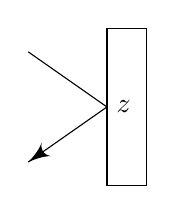
\begin{tikzpicture}
    \draw (1, 1) rectangle (1.5, -1);
    \node at (1, 0) [right] {$z$};
    \draw [->] (0, 0.7) -- (1, 0) -- (0, -0.7);
  \end{tikzpicture}
\end{center}
We see that the light ray travels towards the mirror, gets reflected at $z$, and hits the (invisible) eye. What determines the path? ie. the point $z$ on the mirror? This was answered by Alexandra - the light takes the shortest path. This is a principle, and we use this principle to derive the answer. For example, if $L(z)$ is the length of the path, as a function of $z$, we can solve for $z$ by setting $L'(z) = 0$.

This sounds reasonable - in the absence of mirrors, light travels in a straight line - which is the shortest path between two points.

But is this true? No! Not always. We only considered a plane mirror, and this doesn't hold in we have, say, a spherical mirror. However, it turns out that in all cases, $L'(z) = 0$.

If light travels at finite speed, then the shortest path is the path that gives the minimum time. This is Fermat's principle:
\begin{center}
  Light travels on path that takes the shortest time.
\end{center}
This applies to refraction as well - light rays change direction when travelling between different mediums because they have different speeds in different mediums.

We usually define the refractive index $n$ of a medium to be $n = 1/v$, where $v$ is the velocity of light in the medium. Then we can write the variational principle as
\begin{center}
  maximize $\displaystyle \int_{\text{path}} n\;\d s$,
\end{center}
where $\d s$ is the path length element. This is easy if we have two distinct mediums as above. If $n$ is continuously varying, we need new maths tools - calculus of variations. 

Consider a different problem - Dido's problem. We want to enclose as much area as we wish using a strip of length $L$. We cannot solve this using ordinary calculus. We have an infinite number of paths to try!

We can approximate this by having $n$ pegs on the strip, producing a $n$-gon, and try to maximize it. Then we take $n\to \infty$ and solve our original problem!

\section{Calculus for functions of many variables}
Let $f: \R^n \to \R$ with $\mathbf{x} \mapsto f(\mathbf{x})$. We write $\mathbf{x} = (x_1, \cdots, x_n)$. We assume that $f$ is sufficiently smooth ($C^2(\R)$, ie. twice differentiable, is usually sufficient).  
\begin{defi}[Stationary points]
  \emph{Stationary points} are points in $\R^n$ for which $\nabla f = 0$, ie.
  \[
    \frac{\partial f}{\partial x_1} = \frac{\partial f}{\partial x_2} = \cdots = \frac{\partial f}{\partial x_n} = 0
  \]
\end{defi}
These are not necessarily maximum/minimum. So we expand $f$ in Taylor series about a stationary point $\mathbf{x} = \mathbf{a}$:
\begin{align*}
  f(\mathbf{x}) &= f(\mathbf{a}) + (x - a)\cdot \nabla f + \frac{1}{2}\sum_{i, j}(x_i - a_i)(x_j - a_j)\frac{\partial^2 f}{\partial x_i \partial x_j} + O(x^3).\\
  &= f(\mathbf{a}) + \frac{1}{2}\sum_{i, j}(x_i - a_i)(x_j - a_j)\frac{\partial^2 f}{\partial x_i \partial x_j} + O(x^3).
\end{align*}
The second term is so important that we have a name for it:
\begin{defi}[Hessian matrix]
  The \emph{Hessian matrix} is
  \[
    H_{ij}(x) = \frac{\partial^2 f}{\partial x_i \partial x_j}
  \]
\end{defi}
Of course, we are lazy and choose coordinates such that $\mathbf{a} = \mathbf{0}$. Then
\[
  f(\mathbf{x}) - f(\mathbf{0}) = \frac{1}{2}x_i H_{ij}x_j + O(x^3),
\]
using the summation convention. Since $H$ is symmetric, by rotation of axes, we can diagonalize the quadratic form. Then
\[
  \frac{1}{2}x_i H_{ij}x_j = \frac{1}{2}x_i' H_{ij}'x_j'
\]
with
\[
  H_{ij}' = 
  \begin{pmatrix}
    \lambda_1 & 0 & \cdots & 0\\
    0 & \lambda_2 & \cdots & 0\\
    \vdots & \vdots & \ddots & 0\\
    0 & 0 & \cdots & \lambda_n
  \end{pmatrix}
\]
Since $H$ is symmetric real, the eigenvalues $\lambda_i$ are all symmetric real. Then
\[
  f(\mathbf{x}) - f(\mathbf{0}) = \frac{1}{2}\sum_{i = 0}^n \lambda_i (x_i')^2
\]
Note that this is $\geq 0$ if $\lambda_i > 0$ for all $i$. In this case, stationary point is a local minimum. Similarly, if $\lambda_i < 0$ for all $i$, it is a local minimum. If the eigenvalues have mixed sign, then we go up in some directions, down in others. So we have a saddle point.

If some $\lambda = 0$, we have a \emph{degenerate stationary point}. Here we are in deep, \emph{deep} trouble and have to look at higher derivatives.

\begin{eg}
  Take the boring case where $n = 2$. Then $\det H = \lambda_1, \lambda_2$ and $\tr H = \lambda_1 + \lambda_2$. If $\det H > 0$, then both eigenvalues have same sign. If $\tr H > 0$, both are positive and it is a local minimum. If $\tr H < 0$, it is a local maximum.

  If $\det H < 0$, then the eigenvalues have mixed sign, and it is a saddle. if $\det H = 0$, then it is degenerate.

  For example, let $f(x, y) = x^3 + y^3 - 3xy$. Then
  \[
    \nabla f = 3(x^2 - y, y^2 - x).
  \]
  This is zero iff $x^2 = y$ and $y^2 = x$. So $y^4 = y$. Either $y = 0$, or $y^3 = 1$, ie. $y = 1$. So there are two stationary points: $(0, 0)$ and $(1, 1)$.

  The Hessian matrix is
  \[
    H = 
    \begin{pmatrix}
      6x & -3\\
      -3 & 6y
    \end{pmatrix}
  \]
  So
  \begin{align*}
    \det H &= 9(4xy - 1) = \lambda_1\lambda_2\\
    \tr H &= 6(x + y) = \lambda_1 + \lambda_2
  \end{align*}
  At $(1, 1)$, $\det H > 0$, $\tr H > 0$. So this is a local minimum. At $(0, 0)$, $\det H < 0$. So this is a saddle point.
\end{eg}
\subsection{Convex functions}
\begin{defi}[Convex set]
  A set $S\subseteq \R^n$ is \emph{convex} if for any distinct $\mathbf{x}, \mathbf{y}\in X, t\in (0, 1)$, we have $(1 - t)\mathbf{x} + t\mathbf{y} \in S$. Alternatively, any line joining two points in $S$ lies completely within $S$.

  \begin{center}
    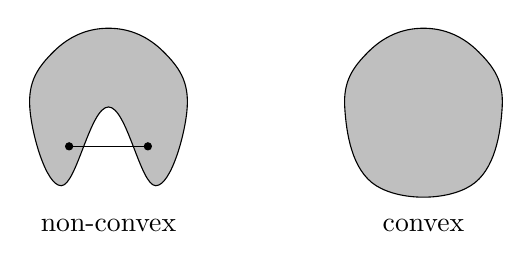
\begin{tikzpicture}
      \begin{scope}[shift={(-2, 0)}]
        \draw [fill=gray!50!white] plot [smooth cycle, tension=0.7] coordinates {(0, 1) (-0.7, 0.7) (-1, 0) (-0.6, -1) (0, 0) (0.6, -1) (1, 0) (0.7, 0.7)};
        \draw (-0.5, -0.5) node [circ] {} -- (0.5, -0.5) node [circ] {};

        \node at (0, -1.5) {non-convex};
      \end{scope}

      \begin{scope}[shift={(2, 0)}]
        \draw [fill=gray!50!white] plot [smooth cycle, tension=0.7] coordinates {(0, 1) (-0.7, 0.7) (-1, 0) (-0.6, -1) (0.6, -1) (1, 0) (0.7, 0.7)};
        \node at (0, -1.5) {convex};
      \end{scope}
    \end{tikzpicture}
  \end{center}
\end{defi}

\begin{defi}[Convex function]
  A function $f: \R^n \to \R$ is \emph{convex} if
  \begin{enumerate}
    \item The domain $D(f)$ is convex
    \item The function $f$ lies below (or on) all its chords, ie.
      \[
        f((1 - t)\mathbf{x} + t\mathbf{y}) \leq (1 - t)f(\mathbf{x}) + tf(\mathbf{y}). \tag{$*$}
      \]
  \end{enumerate}
  A function is \emph{strictly convex} if the inequality is strict, ie.
  \[
    f((1 - t)\mathbf{x} + t\mathbf{y}) < (1 - t)f(\mathbf{x}) + tf(\mathbf{y}).
  \]
  for all $t\in (0, 1)$.
  \begin{center}
    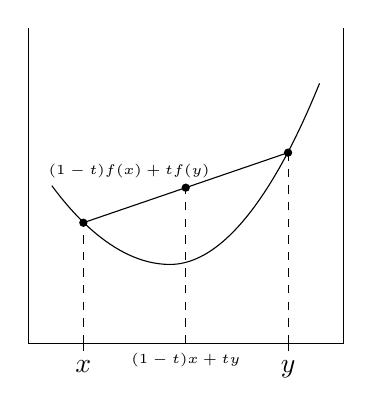
\begin{tikzpicture}
      \draw(-2, 4) -- (-2, 0) -- (2, 0) -- (2, 4);
      \draw (-1.3, 0.1) -- (-1.3, -0.1) node [below] {$x$};
      \draw (1.3, 0.1) -- (1.3, -0.1) node [below] {$y$};
      \draw (-1.7, 2) parabola bend (-.2, 1) (1.7, 3.3);
      \draw [dashed] (-1.3, 0) -- (-1.3, 1.53) node [circ] {};
      \draw [dashed] (1.3, 0) -- (1.3, 2.42) node [circ] {};
      \draw (-1.3, 1.53) -- (1.3, 2.42);
      \draw [dashed] (0, 0) node [below] {\tiny $(1 - t)x + ty$} -- (0, 1.975) node [above] {\tiny$(1 - t)f(x) + t f(y)\quad\quad\quad\quad\quad\quad$} node [circ] {};
    \end{tikzpicture}
  \end{center}

  A function $f$ is (strictly) concave iff $-f$ is (strictly) convex.
\end{defi}

\begin{eg}\leavevmode
  \begin{enumerate}
    \item $f(x) = x^2$ is strictly convex.
    \item $f(x) = |x|$ is convex, but not strictly
    \item $f(x) = \frac{1}{x}$ defined on $x > 0$ is strictly convex.
    \item $f(x) = \frac{1}{x}$ defined on $\R^* = \R \setminus \{0\}$ is \emph{not} convex. Apart from the fact that $\R^*$ is not a convex domain. But even if we defined, like $f(0) = 0$, it is not convex by considering the line joining $(-1, -1)$ and $(1, 1)$ (and in fact $f(x) = \frac{1}{x}$ defined on $x < 0$ is concave).
  \end{enumerate}
\end{eg}
\subsubsection{First-order convexity condition}
Now assume that the function is differentiable. Then we have the first-order condition for convexity. Assume $f$ is (at least) once-differentiable. It is convex if
\[
  h(t) = (1 - t)f(\mathbf{x}) + tf(\mathbf{y}) - f((1 - t)\mathbf{x} + f(\mathbf{y})) \geq 0.
\]
We have $h(0) = 0$. So
\[
  \frac{h(t) - h(0)}{t} \geq 0
\]
for any $t\in (0, 1)$. So
\[
  h'(0) \geq 0.
\]
On the other hand,
\[
  h'(0) = f(\mathbf{y}) - f(\mathbf{x}) - (\mathbf{y} - \mathbf{x})\nabla f (\mathbf{x}).
\]
So convexity implies that
\[
  f(\mathbf{y}) \geq f(\mathbf{x}) + (\mathbf{y} - \mathbf{x})\nabla f(\mathbf{x}) \tag{$\dagger$}
\]
It is also true that $(\dagger)\Rightarrow (*)$, which is an easy exercise. So a convex differentiable function lies above all its tangent planes.

\begin{cor}
  A stationary point of a convex function is a global minimum. There can be more than one global minimum (eg a constant function), but there is at most one if the function is strictly convex.
\end{cor}

\begin{proof}
  Given $\mathbf{x}_0$ such that $\nabla f(\mathbf{x}_0) = \mathbf{0}$, $(\dagger)$ implies that for any $\mathbf{y}$,
  \[
    f(\mathbf{y}) \geq f(\mathbf{x_0}) + (\mathbf{y} - \mathbf{x}_0)\nabla f(\mathbf{x}_0) = f(\mathbf{x}_0).
  \]
\end{proof}

We can rewrite $(\dagger)$ to say
\[
  (\mathbf{y} - \mathbf{x}) \cdot [\nabla f(\mathbf{y}) - \nabla f(\mathbf{x})] \geq f(\mathbf{x}) - f(\mathbf{y}) - (\mathbf{x} - \mathbf{y}) \cdot \nabla f(\mathbf{y}).
\]
But the right is $\geq 0$ by $\dagger$. So we have another first-order condition:
\[
  (\mathbf{y} - \mathbf{x})\cdot [\nabla f(\mathbf{y}) - \nabla f(\mathbf{x})]  \geq 0,
\]
It can be shown that this is equivalent to the other conditions.

This should be interpreted as ``$\nabla f(\mathbf{x})$ is a non-decreasing function''. For example, when $n = 1$, we have $(y - x)(f'(y) - f'(x)) \geq 0$, which implies that $f'(y) > f'(x)$ for $y > x$.

\subsubsection{Second-order convexity condition}
Assume that $f$ is (at least) twice differentiable.

In the last condition we had, let $\mathbf{y} = \mathbf{x} + \mathbf{h}$. Then
\[
  \mathbf{h} \cdot (\nabla f(\mathbf{x} + \mathbf{h}) - \nabla f(\mathbf{x})) \geq 0.
\]
Expand the left in Taylor series. Then the left hand side is
\[
  h_i [h_j \nabla_j \nabla_i f + O(h^2)]
\]
But $\nabla_j \nabla_i f = H_{ij}$. So we have
\[
  h_i H_{ij}h_j + O(h^3) \geq 0
\]
This is true for all $h$ if the Hessian $H$ is positive, ie. the eigenvalues are non-negative. If they are in fact all positive, then we say $H$ is positive definite.

Hence convexity implies that the Hessian matrix is positive for all $\mathbf{x}\in D(f)$. Strict convexity implies that it is positive definite.

The converse is also true - if the Hessian is positive definite, then it is convex.

\begin{eg}
  Let $f(x, y) = \frac{1}{xy}$ for $x, y > 0$. Then the Hessian is
  \[
    H = \frac{1}{xy}
    \begin{pmatrix}
      \frac{2}{x^2} & \frac{1}{xy}\\
      \frac{1}{xy} & \frac{2}{y^2}
    \end{pmatrix}
  \]
  The determinant is
  \[
    \det H = \frac{3}{x^4y^4} > 0
  \]
  and the trace is
  \[
    \tr H = \frac{2}{xy}\left(\frac{1}{x^2} + \frac{1}{y^2}\right) > 0.
  \]
  So $f$ is convex.

  We only relied on $xy$ being positive. Can we relax the domain condition to be $xy > 0$ instead? No! This is because the domain will no longer be convex! 
\end{eg}

\subsection{Legendre transform}
\begin{defi}[Legendre transform]
  Given a function $f: \R^n \to \R$, its \emph{Legendre transform} $f^*$ (the ``conjugate'' function) is defined by
  \[
    f^*(\mathbf{p}) = \sup_{x}(\mathbf{p}\cdot \mathbf{x} - f(\mathbf{x})),
  \]
  The domain of $f^*$ is the set of $\mathbf{p}\in \R^n$ such that the supremum is finite.
\end{defi}
It follows immediately that
\begin{lemma}
  $f^*$ is always convex.
\end{lemma}

\begin{proof}
  \begin{align*}
    f^*((1 - t)\mathbf{p} + t\mathbf{q}) &= \sup_x \big[((1 - t)\mathbf{p}\cdot \mathbf{x} + t\mathbf{q}\cdot \mathbf{x} - f(\mathbf{x})\big].\\
    &= \sup_x \big[(1 - t)(\mathbf{p}\cdot \mathbf{x} - f(\mathbf{x})) + t(\mathbf{q}\cdot \mathbf{x} - f(\mathbf{x}))\big]\\
    &\leq (1 - t)\sup_x [\mathbf{p}\cdot \mathbf{x} - f(\mathbf{x})] + t\sup_x[\mathbf{q}\cdot \mathbf{x}  - f(\mathbf{x})]\\
    &= (1 - t)f^*(\mathbf{p}) + tf^*(\mathbf{q})\\
  \end{align*}
  Note that we cannot immediately conclude that $f$ is convex, since we have to show that the domain is convex. But by the above bounds, $f^*((1 - t)\mathbf{p} + t\mathbf{q})$  is bounded by the sum of two finite terms, which is finite. So $(1 - t)\mathbf{p} + t\mathbf{q}$ is also in the domain of $f$.
\end{proof}

Now suppose that $f(\mathbf{x})$ is differentiable. Then the maximum of the right hand side is found by solving (for $\mathbf{x}$ as a function of $\mathbf{p}$) $\mathbf{p} = \nabla f(\mathbf{x})$

If $f$ is strictly convex, then a solution of this equation (if exists) is unique.

For example, when $n = 1$, $f^*(p) = px - f(x)$, where $x$ satisfies $f'(x) = p$.

\begin{center}
  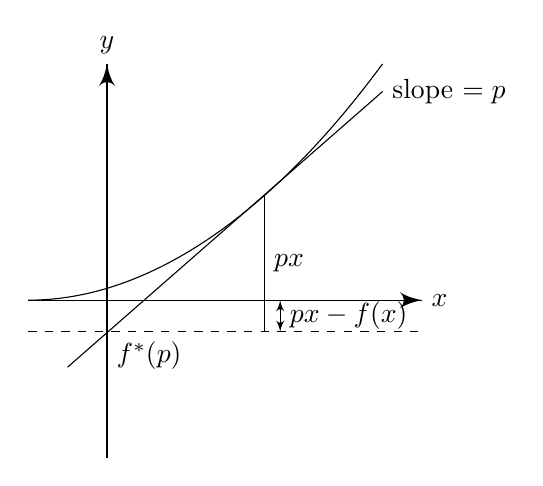
\begin{tikzpicture}
    \draw [->] (-1, 0) -- (4, 0) node [right] {$x$};
    \draw [->] (0, -2) -- (0, 3) node [above] {$y$};
    \draw (-1, 0) parabola (3.5, 3);
    \draw (3.5, 2.65) node [right] {slope $=p$} -- +(-4, -3.5);
    \draw [dashed] (-1, -0.4) -- +(5, 0);
    \node at (0, -0.4) [anchor = north west] {$f^*(p)$};
    \draw (2, -0.4) -- +(0, 1.74) node [pos=0.5, right] {$px$};
    \draw [arrows={latex'-latex'}] (2.2, 0) -- (2.2, -0.4) node [right, pos=0.5] {$px - f(x)$};
  \end{tikzpicture}
\end{center}

\begin{eg}\leavevmode
  \begin{enumerate}
    \item Let $f(x) = \frac{1}{2}ax^2$ for $a > 0$. Then $p = ax$ at the maximum of $px - f(x)$. So
      \[
        f^*(p) = px - f(x) = p\cdot \frac{p}{a} - \frac{1}{2}a\left(\frac{p}{a}\right)^2 = \frac{1}{2a}p^2.
      \]
      So the Legendre transform maps a parabola to a parabola.
    \item $f(v) = -\sqrt{1 - v^2}$ for $|v| < 1$ is a lower semi-circle. We have
      \[
        p = f'(v) = \frac{v}{\sqrt{1 - v^2}}
      \]
      So
      \[
        v = \frac{p}{\sqrt{1 + p^2}}
      \]
      and exists for all $p\in \R$. So
      \[
        f^*(p) = pv - f(v)|_{v = v(p)} = \frac{p^2}{\sqrt{1 + p^2}} + \frac{1}{\sqrt{1 + p^2}} = \sqrt{1 + p^2}.
      \]
      A circle gets mapped to a hyperbola.
    \item Let $f = cx$ for $c > 0$. This is convex but not strictly convex. Then $px - f(x) = (p - c)x$. This has no maximum unless $p = c$. So the domain of $f^*$ is simply $\{c\}$. One point. So $f^*(p) = 0$. So a line goes to a point.
  \end{enumerate}
\end{eg}
\begin{thm}
  If $f$ is convex, differentiable with Legendre transform $f^*$, then $f^{**} = f$. 
\end{thm}

\begin{proof}
  We have $f^*(\mathbf{p}) = (\mathbf{p}\cdot\mathbf{x}(\mathbf{p}) - f(\mathbf{x}(\mathbf{p}))$ where $\mathbf{p} = \nabla f(\mathbf{x}(\mathbf{p}))$.

  Differentiating with respect to $\mathbf{p}$, we have
  \begin{align*}
    \nabla_i f^*(\mathbf{p}) &= x_i + p_j \nabla_i x_j (\mathbf{p}) - \nabla_i x_j(\mathbf{p}) \nabla_j f(\mathbf{x})\\
    &= x_i + p_j \nabla_i x_j(\mathbf{p}) - \nabla_i x_j(\mathbf{p}) p_j\\
    &= x_i.
  \end{align*}
  So
  \[
    \nabla f^*(\mathbf{p}) = \mathbf{x}.
  \]
  Hence
  \begin{align*}
    \nabla f(\mathbf{x}) = \mathbf{p} &\Rightarrow \mathbf{x} = \mathbf{x}(\mathbf{p})\\
    \nabla f^*(\mathbf{p}) = \mathbf{x} &\Rightarrow \mathbf{p} = \mathbf{p}(\mathbf{x}).
  \end{align*}
  Now we take the Legendre transform of $f^*$:
  \begin{align*}
    f^{**}(\mathbf{x}) &= (\mathbf{x} \cdot \mathbf{p} - f^*(\mathbf{p}))|_{\mathbf{p} = \mathbf{p}(\mathbf{x})}\\
    &= \mathbf{x}\cdot \mathbf{p} - (\mathbf{p}\cdot \mathbf{x} - f(\mathbf{x}(\mathbf{p}(\mathbf{x}))))\\
    &= f(\mathbf{x}).
  \end{align*}
\end{proof}
\note if $f = (f^*)^*$, then $f$ is convex since it is a Legendre transform. So the convexity condition is really required for the theorem.

Note that strict convexity is \emph{not} required. For example, in our last example above, $f^*(p) = 0$ for $p = c$. So $f^{**}(x) = (xp - f^*(p))|_{p = c} = cx = f(x)$.

\subsection{Application to thermodynamics}
For a system in thermal equilibrium at temperature $T$ and pressure $P$, the first law of thermodynamics says that
\[
  \d E = T\;\d S - p\;\d V.
\]
Here $T\;\d S = \d Q$ is the heat change, and $-p\;\d V = \d W$ is the work done.

From this, we obtain
\[
  \frac{\partial E}{\partial S} = T,\quad \frac{\partial E}{\partial V} = p
\]
We say that $S$ and $V$ \emph{extensive} variables - they scale with the system; $T$ and $p$ are \emph{intensive} variables.

On the right hand side of the first law, variables come in conjugate pairs, eg. $(T, S)$, $(p, V)$. In other cases, we have like $(\mu, N)$, the chemical potential and number of particles.

To find the equilibrium at fixed $S$, we minimize $E$. But in practice, we fix $T$ and not $S$, ie. we put in contact with a heat reservoir.

In this case, it is the \emph{Helmholtz free energy}
\[
  F(T, V) = E(S, V) - TS = E(S, V) - S\frac{\partial E}{\partial S}.
\]
that is minimized. We see that $F(T, V)$ is the Legendre transform of $-E(S, V)$.

If we get the Legendre transform with respect to $V$, we get the enthalpy instead.

\section{Lagrange multipliers}
Let $f(x, y)$ be the height above ground. The hill tip is at the max of $f$, which satisfies
\[
  0 = \d f = \nabla f\cdot \d \mathbf{\ell}
\]
for all $\d \mathbf{\ell}$. So we need
\[
  \nabla f = 0.
\]
However, suppose we have a particular path $p$ defined by $p(x, y) = 0$. Where is the highest point on the path $p$?

We still need $\nabla f \cdot \d \mathbf{\ell} = 0$, but now $\d \mathbf{\ell}$ is \emph{not} arbitrary, but only for $\d \ell$ that is parallel to the path. Alternatively, $\nabla f$ has to be entirely perpendicular to the path. Since we know that the normal to the path is $\nabla p$, our condition becomes
\[
  \nabla f = \lambda \nabla p
\]
for some lambda $\lambda$. Of course, we still have the constraint $p(x, y) = 0$. So what we have to solve is
\begin{align*}
  \nabla f &= \lambda \nabla p\\
  p &= 0
\end{align*}
for the three variables $x, y, \lambda$.

Alternatively, we can solve for the stationary points of the function $\phi(x, y, \lambda)$ given by
\[
  \phi(x, y, \lambda) = f(x, y) - \lambda p(x, y)
\]
Now we have changed constrained maximization problem to a problem of unconstrained extremization.

\begin{eg}
  Find the radius of the smallest circle centered on origin that intersects $y = x^2 - 1$.

  \begin{enumerate}
    \item  First do it the easy way: for a circle of radius $R$ to work, $x^2 + y^2 = R^2$ and $y = x^2 - 1$ must have a solution. So
      \[
        (x^2)^2 - x^2 + 1 - R^2 = 0
      \]
      and
      \[
        x^2 = \frac{1}{2}\pm \sqrt{R^2 - \frac{3}{4}}
      \]
      So $R_{\min} = \sqrt{3}/2$.

    \item We can also view this as a variational problem. We want to minimize $f(x, y) = x^2 + y^2$ subject to the constraint $p(x, y) = 0$ for $p(x, y) = y - x^2 + 1$.

      We can solve this directly. We can solve the constraint to obtain $y = x^2 - 1$. Then 
      \[
        R^2(x) = f(x, y(x)) = (x^2)^2 - x^2  + 1
      \]
      We look for stationary points of $R^2$:
      \[
        (R^2(x))' = 0 \Rightarrow  x\left(x^2 - \frac{1}{2}\right)= 0
      \]
      So $x = 0$ and $R = 1$; or $x = \pm \frac{1}{\sqrt{2}}$ and $R = \frac{\sqrt{3}}{2}$. Since $\frac{\sqrt{3}}{2}$ is smaller, this is our minimum.

    \item Finally, we can use Lagrange multipliers. We find stationary points of the function 
      \[
        \phi(x, y, \lambda) = f(x, y) - \lambda p(x, y) = x^2 + y^2 - \lambda (y - x^2 + 1)
      \]
      The partial derivatives give
      \begin{align*}
        \frac{\partial \phi}{\partial x} = 0 &\Rightarrow 2x(1 + \lambda) = 0\\
        \frac{\partial \phi}{\partial y} = 0 &\Rightarrow 2y - \lambda = 0\\
        \frac{\partial \phi}{\partial \lambda} = 0 &\Rightarrow y - x^2 + 1 = 0
      \end{align*}
      The first equation gives us two choices: If $x = 0$, then $y = -1$. So $\lambda = -1$. Then $R = 1$.

      If $\lambda = -1$, we have $y = -\frac{1}{2}$ and $x = \pm \frac{1}{\sqrt{2}}$. So $R = \frac{\sqrt{3}}{2} < 1$ is the minimum.
  \end{enumerate}
\end{eg}
This can be generalized to problems with functions $\R^n \to \R$ using the same logic.

\begin{eg}
  For $x\in \R^n$, find the minimum of the quadratic form
  \[
    f(x) = x_i A_{ij}x_j
  \]
  on the surface $|\mathbf{x}|^2 = 1$.

  \begin{enumerate}
  \item The constraint imposes a normalization condition $\mathbf{x}$. But if we scale up $\mathbf{x}$, $f(\mathbf{x})$ scales accordingly. So if we define
    \[
      \Lambda(\mathbf{x}) = \frac{f(\mathbf{x})}{g(\mathbf{x})},\quad g(\mathbf{x}) = |\mathbf{x}|^2
    \]
    The problem is equivalent to minimization of $\Lambda (\mathbf{x})$ without constraint. Then
    \[
      \nabla_i \Lambda(\mathbf{x}) = \frac{2}{g}\left[A_{ij} x_j - \frac{f}{g} x_i\right]
    \]
    So we need
    \[
      A\mathbf{x} = \Lambda \mathbf{x}
    \]
    So the extremal values of $\Lambda (\mathbf{x})$ are the eigenvalues of $A$. If $A$ is positive, then $\Lambda_{\min}$ is the lowest eigenvalue.

  \item We can also do it with Lagrange multipliers. We want to find stationary values of 
    \[
      \phi(\mathbf{x}, \lambda) = f(\mathbf{x}) - \lambda(|\mathbf{x}|^2 - 1).
    \]
    So
    \[
      0 = \nabla \phi \Rightarrow  A_{ij} x_j = \lambda x_i
    \]
    Differentiating with respect to $\lambda$ gives
    \[
      \frac{\partial \phi}{\partial \lambda} = 0 \Rightarrow  |\mathbf{x}|^2 = 1.
    \]
    So we get the same set of equations.
  \end{enumerate}
\end{eg}

\begin{eg}
  What probability distribution $\{p_1, \cdots, p_n\}$ satisfying $\sum_i p_i = 1$ maximizes the information entropy
  \[
    S = - \sum_{i = 1}^n p_i \log p_i
  \]
  We look for stationary points of
  \[
    \phi(\mathbf{p}, \lambda) = -\sum_{i = 1}^n p_i \ln p_i - \lambda\sum_{i = 1}^n p_i + \lambda.
  \]
  We have
  \[
    \frac{\partial \phi}{\partial p_i}= - \ln p_i - (1 + \lambda) = 0
  \]
  So
  \[
    p_i = e^{-(1 + \lambda)}
  \]
  It's the same for all $i$! So we must have $p_i = \frac{1}{n}$.
\end{eg}
\end{document}
